% Mit folgendem Header kann ich wahlweise 'latex bla.tex', oder 'pdflatex
% bla.tex' laufen lassen. Es wird dann eine dvi bzw. pdf Datei erzeugt. Die
% Bilder, die mit includegraphics importiert werden, werden ohne Dateiendung
% angegeben. Latex sucht sich dann entweder ein .eps bzw. .pdf/.png/.jpg File
% heraus...
%
%(http://www.techfak.uni-bielefeld.de/ags/ni/lectures/internstuff/howto/howto-la
%tex/howto-pdflatex.html)
\newif\ifpdf \ifx\pdfoutput\undefined
\pdffalse % we are not running pdflatex
\else
\pdfoutput=1 % we are running pdflatex
\pdfcompresslevel=9 % compression level for text and image;
\pdftrue \fi

\documentclass[12pt, headsepline]{scrreprt}
\usepackage[ngerman]{babel}

\ifpdf
  \usepackage[pdftex,xdvi]{graphicx}
  \usepackage[pdftex]{hyperref}         % option [colorlinks] erzeugt farbige Links statt

  \pdfinfo{
     /Title    (Abschlussbericht Muminav)
     /Author   (Michael Gl�ssel, Matthias Erche, J�rg K�ster)
     /Subject  ()
     /Keywords (tu-berlin, open source, java)
  }
  \usepackage[pdftex]{color}            % farbige Umrandungen
\else
  \usepackage[dvips,xdvi]{graphicx}
  \usepackage[colorlinks]{hyperref}
  \usepackage{color}
\fi

\usepackage[automark,headsepline,plainheadsepline]{scrpage2}
\pagestyle{scrheadings}
%\ohead[\pagemark]{\pagemark}
\ohead[\headmark]{\headmark} \chead{\empty}


% ersetzt, s. o.
% \usepackage{color}                    % um den Text auch farbig zu gestalten
% \usepackage[dvips]{graphicx}          % zum Einbinden von Grafiken, [<TREIBER>]

\usepackage{subfigure}                  % mehrere figures in einem floating object
\usepackage[latin1]{inputenc}           % f�r Umlaute
\usepackage{textcomp}                   % fuer Sonderzeichen wie <Grad Celsius>
% \usepackage{hyperref}                 % zum Einbinden von Querverweisen in pdf (als letztes
                                        % auffuehren!)
%\graphicspath{{figs/}}               % jetzt muss man nicht jedesmal den Pfad angeben

\usepackage{array}



\title{Abschlussbericht \\ Muminav}

\author{
  Open-Source-Softwareprojekt\\
  Sommersemester 2002\\
  Technische Universit�t Berlin \\ \\
  \normalsize Michael Gl�ssel \\
  \normalsize Matthias Erche \\
  \normalsize J�rg K�ster\\
}

\date{\today}

\begin{document}                        % here begins the actual document body
%\maketitle                             % this actually creates the title block




\vspace*{\stretch{1}} \rule{\linewidth}{1mm}

\begin{flushright}
    \thispagestyle{empty}
    {\Large \textbf{Abschlu�bericht}\\}
 %   {\Huge \textbf{Muminav}\\}
\begin{figure}[htbp]
    \begin{flushright}
        \includegraphics[width=10cm]{figs/logo}
    \end{flushright}
\end{figure}
    \vspace{0.1cm}
    %\large



\begin{minipage}[b]{13cm}
\begin{raggedleft}
    Im Rahmen der Veranstaltung:\\
    Dezentrale Systementwicklung am Beispiel GNU/LINUX\\
    an der TU-Berlin --
    Sommersemester 2002\\
\end{raggedleft}
\end{minipage}
%\hspace*{21mm}
%\begin{minipage}[b]{\linewidth}
\begin{minipage}[t]{2cm}
\includegraphics[height=1.5cm]{figs/tulogo}
\end{minipage}





%    }

\end{flushright}


\rule{\linewidth}{1mm}





\vspace*{\stretch{2}}
\begin{center}
\large \textsc{Michael Gl\"assel, Matthias Erche, J�rg K�ster} \\
{\normalsize Betreuung: \textsc{Steffen Evers}}\\
\vspace{0.7cm} \today\\
%\begin{figure}[htbp]
%       \centering
%        \includegraphics[width=1.5cm]{figs/tulogo}
%\end{figure}
\end{center}


\begin{abstract}
\textbf{Zusammenfassung} blah \ldots
\end{abstract}

\tableofcontents

%--------------------------------------------------------------------
\chapter{Einleitung}

\section{Der Projektkontext}

Die Arbeit am Projekt Muminav begann im Mai 2002 im Rahmen einer
Lehrveranstaltung an der TU-Berlin\footnote{{http://www.tu-berlin.de}}. Es
handelt sich dabei um die Realisierung eines Teils des ebenfalls an der
TU-Berlin laufenden Projektes  \glqq Multimediale Mathematikausbildung f�r
Ingenieure\grqq\ \footnote{kurz: \textsc{Mumie}} \cite{Mumie}.

\subsection{Dezentrale Systementwicklung am Beispiel GNU/Linux}

Die Lehrveranstaltung \glqq Dezentrale Systementwicklung am Beispiel
GNU/Linux \grqq\ \cite{DESE}, die am Institut f�r
Elektrotechnik und Informatik\footnote{{http://cs.tu-berlin.de}} angeboten wird,
soll den Teilnehmern einen Einblick in die dezentrale Entwicklung von
Softwaresystemen verschaffen. Der Schwerpunkt liegt auf der Betrachtung von Open
Source Software.

Der theoretische Teil umfasst Themen wie die Geschichte und Philosophie von Open
Source Software (im Speziellen GNU/Linux), Parallelen zwischen
Wissenschafts- und Entwicklungstheorien zum Ent- und Bestehen von freien
Softwaresystemen, die Organisation und Eigenheiten entsprechender Projekte und
die damit verbundenen Anforderungen an die Entwickler, Hilfsmittel, die die
dezentrale Entwicklung unterst�tzen und einige andere mehr.

F�r den praktischen Teil bearbeiten die Teilnehmer ein Projekt, um selbst
Erfahrungen auf dem Gebiet der dezentralen Systementwicklung zu sammeln. Es
werden vom Veranstalter Projektphasen vorgegeben, zu denen Vortr�ge und
Ausarbeitungen den Stand der Entwicklung wiederspiegeln sollen. Die Entwicklung
soll durch die Nutzung von in diesem Bereich bekannten Tools (z.B.
Mailinglisten, CVS, Homepage etc.) unterst�tzt werden und es wird die
Wiederbenutzung schon bestehender Software angeregt. Ziel ist es, zum Abschluss
der Veranstaltung einen Prototypen des Systems vorzustellen.

Die Inhalte der Projekte stehen den Teilnehmern v�llig frei. Sie suchen sich
selbst ein Thema oder arbeiten mit einem externen Auftraggeber
zusammen. Daf�r werden auch einige Kontakte vom Veranstalter hergestellt
und angeboten.

\subsection{Das Projekt Mumie}

\glqq Multimediale Mathematikausbildung f�r Ingenieure\grqq\ ist ein vom
Bundesministerium f�r Bildung und Forschung gef�rdertes Projekt, dass an der
TU-Berlin in Kooperation mit 3 weiteren deutschen Universit�ten entwickelt wird.

Das Ziel liegt in der Entwicklung einer WWW-basierten, modularen Umgebung, die
einerseits dem Lernendem den Zugang zur Mathematik und andererseits dem Dozenten
die Vermittlung von Wissen durch den Einsatz moderner, multimedialer
Techniken erleichtern soll. Das System soll aus mehreren Modulen bestehen:

\begin{itemize}
\raggedright
\item Darstellung mathematischer Inhalte mit interaktiver
Multimedia-Unterst�tzung
\item Stoffnachbereitung, Wiederholungsunterst�tzung angeleitete und kommen\-tier\-te
�bungs\-auf\-gaben
\item Selbstkontrolle durch individuelle
Testumgebungen
\item Einf�hrung in mathematische Standardsoftwarepakete
\item individuelles Trainingscenter weiterf�hrender
Inhalte
\item Informationsplattform in der und vile und in die der es auch
noch kein wer, was, wie, wo
\item Kommunikations-- und
Austauschangebote
\end{itemize}

Zus�tzlich werden Schwerpunkte auf eine individualisierbare Oberfl�che und eine
intelligente Benutzerf�hrung gesetzt, um den Benutzern einen einfachen Umgang
mit dem Stoff zu erm�glichen.

\section{Ziele}

Ein Dozent soll die M�glichkeit haben, aus einer Auswahl an
Elementen \footnote{Motivation, Definition, Theorem, Lemma,
Algorithmus, Anwendung}, die in einer Datenbank gespeichert sind,
die Zusammenstellung f�r einen Kurs zu erstellen. Dies soll durch
einfaches Ziehen und Ablegen von Elementsymbolen auf einer
Zeichenfl�che erfolgen. Zusammenh�nge zwischen Elementen werden
dabei durch Verbindungslinien dargestellt, die der Verfasser
positionieren kann. Zus�tzlich kann es zu den Elementen
Subelemente \footnote{Herleitung, Beweis, Motivation, Bemerkung,
Historisches, Visualisierung, Beispiel, Tabelle} geben. Es
entsteht durch die Zusammenstellung eine Repr�sentation der
mathematischen Zusammenh�nge mittels eines gerichteten Graphen.
Der Dozent kann zur Darstellung des Kursverlaufes eine Art \glqq
roten Faden\grqq\ festlegen, der allerdings nicht entlang der
angelegten Verbindungen laufen muss \footnote{Aktueller Stand,
�nderungen m�glich}.

Die Aufgabe f�r das Projekt \textsc{MumiNav} besteht darin, dieses
vorgegebene Netz mit Hilfe eines Java-Applets in einem
Navigationsframe darzustellen und somit den Zugriff auf die
Inhalte zu erm�glichen. Die Darstellung der Elemente erfolgt durch
unterschiedlich farbige, leicht dreidimensional angedeutete
K�sten. Subelemente werden nach vorgeschriebenen Regeln an diesen
K�sten angeordnet und sind standardm��ig nicht mit
Unterscheidungsmerkmalen versehen.

\begin{figure}[htbp]
    \centering%
%   \setcapwidth[c]{12cm}%
    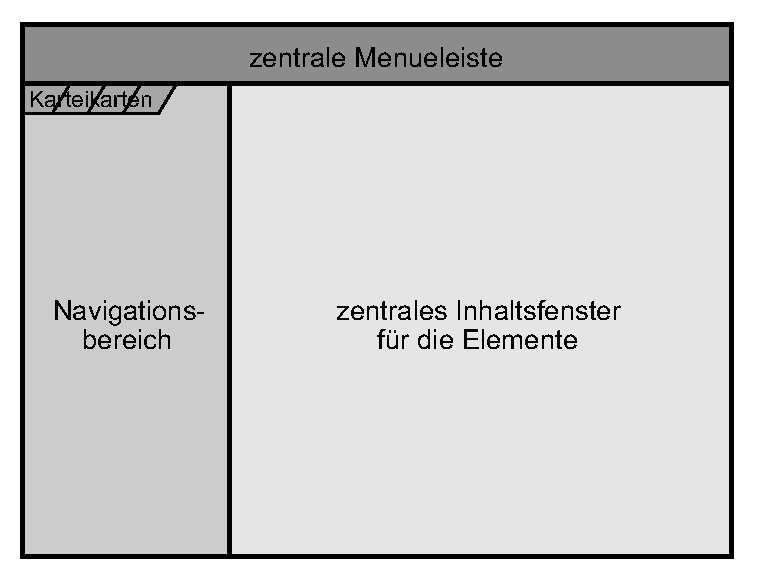
\includegraphics[width=8cm]{figs/haupframe}
    \captionbelow{Layout der Hauptansicht }
    \label{FIG:Hauptansicht}
\end{figure}

Die Abbildung des logischen Netzes geschieht, wie vorher
beschrieben, durch Verbindungslinien zwischen den Elementsymbolen.
Es wird ein \glqq roter Faden\grqq\ entsprechend der linearen
Anordnung der Kursinhalte gelegt.

\begin{figure}[htbp]
    \centering%
%   \setcapwidth[c]{12cm}%
    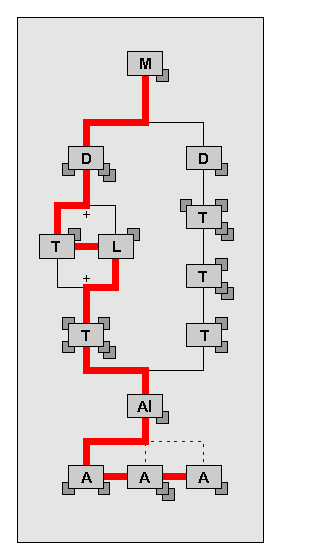
\includegraphics[height=7cm]{figs/navinetz}
    \captionbelow{Kurspfade und roter Faden}
    \label{FIG:roterFaden}
\end{figure}

Die Darstellung soll auf mehrere Maus-Aktionen reagieren. Wird die
Maus �ber ein Element bewegt, soll dieses vergr��ert dargestellt
werden und die Subelemente werden unterscheidbar durch
Beschriftung. Bei Klick mit der linken Maustaste soll der Inhalt
des jeweiligen (Sub-)Elementes im zentralen Inhaltsfenster
dargestellt werden. Dieselbe Aktion auf der mittleren Maustaste
f�hrt zu einem �ffnen des Inhalts in einem externen Fenster und
schlie�lich ist es zuk�nftig vorgesehen, mit der rechten Maustaste
eine Liste von Optionen anzubieten.

\begin{figure}[htbp]
    \centering%
%   \setcapwidth[c]{12cm}%
    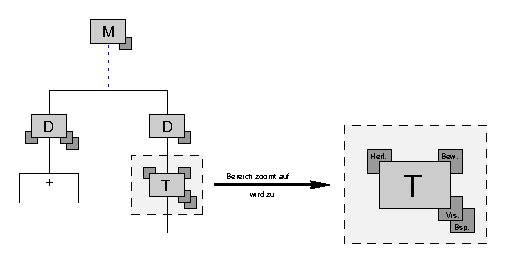
\includegraphics[width=10cm]{figs/zoom_element}
    \captionbelow{Detailansicht bei Zoom}
    \label{FIG:zoomElement}
\end{figure}


\chapter{Organisation des Gesamtprojekts}

An \textsc{Muminav} haben im Rahmen der Veranstaltung
\emph{Dezentrale Systementwicklung am Beispiel GNU/LINUX}
mitgewirkt: J�rg K�ster, Matthias Erche und Michael Gl�ssel. Alle,
Studenten der TU-Berlin im Fach Informatik.

\section{Meilensteine}

Die Termin- und Sachzielverfolgung wurde mit Hilfe von 4
Meilensteinen sichergestellt.

\begin{itemize}
\item \textbf{8.\ Mai} Festlegung auf eine Projektaufgabe
\item \textbf{29.\ Mai} Bestandsaufnahme von relevanten Projekten
\item \textbf{19.\ Juni} Vorlage des L�sungskonzept
\item \textbf{1.\ Oktober} Zwischenbilanz und Prototyp
\end{itemize}



\section{Workshops}

Beim Workshop, der am 10.\ Juli stattfand, ging es um die
Nachbearbeitung, Analyse und Erg�nzung der gesammelten
Erfahrungen. Dazu wurden Gastredner eingeladen, die sich seit
l�ngerer Zeit in diesem Bereich bet�tigen und die mit ihrem Wissen
dazu beitragen k�nnen, die pers�nlichen Erfahrungen der Teilnehmer
in einem allgemeineren und objektiverem Zusammenhang zu sehen.


\section{Gruppenaufteilung}


Die Entwicklungs- und Implementierungsarbeit hat sich wie folgt
aufgeteilt:

\begin{itemize}
    \item \textbf{Matthias Erche} Entwerfen des Desings und der Inhalte der
    Projekt-Homepage, XML-Treeparser, Datenaustauschformat
    \item \textbf{J�rg K�ster} Zoomfunktionalit�t, Dokumentation
    und Skins
    \item \textbf{Michael Gl�ssel} Entwicklung des Grundger�sts,
    Mouseoververhalten und Tooltips
\end{itemize}

Zu jedem der ersten drei Meilensteine hat ein Gruppenmitglied
einen Vortrag gehalten.


\chapter{Muminav -- Die Umsetzung}
In den folgenden Kapiteln m�chten wir einerseits einen �berblick �ber die
technische Realisierung des Projektes geben, aber auch einen Eindruck der
Entwicklungsmodalit�ten und der n�tigen �berlegungen, die bei der Realisierung
eines Open Source Projektes n�tig sind, vermitteln.

\section{Lizenz}

Eine Vorgabe f�r die Entwicklung war, die gesamte Arbeit als Open
Source Projekt durchzuf�hren. Dies schlie�t ein, die
Projektergebnisse unter einer Open Source Lizenz \cite{OSI2002} zu
ver�ffentlichen.

Zur Diskussion standen zwei Lizenzen. Die GPL \cite{GPL1991} (GNU General Public
License), als eine der meistverwendeten Lizenzen im Open Source Bereich, sieht
vor, eine Software f�r jeden frei verf�gbar, nutzbar und ver�nderbar zu machen.
Hinzu kommt der Aspekt, dass Programme, die GPL lizensierte Software benutzen
(linken) oder die durch die Weiterentwicklung dieser entstehen, wieder unter
der GPL stehen m�ssen. So wird verhindert, dass man von der Arbeit anderer
profitiert, ohne eine Gegenleistung zu erbringen.

Eine Lockerung dieser Politik sieht die LGPL \cite{LGPL1999} (Lesser General
Public License oder auch Library General Public License) vor. Urspr�nglich
eingef�hrt, um das Linken von frei verf�gbaren Bibliotheken aus propriet�ren
Systemen heraus zu erm�glichen, ohne Einfluss auf die urspr�ngliche Lizenz zu
nehmen, wird sie heutzutage �berall dort verwendet, wo freie Software auch in
kommerziellen und nicht freien Umgebungen eingesetzt wird.

Da der Ursprung von \textsc{MumiNav} in der Entwicklung eines Navigationssystems
f�r die modulare Lernumgebung \textsc{Mumie} liegt, musste bei der Wahl der
Lizenz darauf R�cksicht genommen werden. Zum Entstehungszeitpunkt dieses
Dokumentes wird zwar f�r die \textsc{Mumie} ebenfalls eine Open Source Lizenz
vorgesehen, doch ist in Zukunft ein kommerzieller Einsatz nicht ausgeschlossen.

Um eventuelle Vorhaben in dieser Richtung nicht zu verhindern, haben wir uns
deshalb dazu entschlossen, \textsc{MumiNav} unter die LGPL zu stellen und somit
die freie Verf�g- und Benutzbarkeit zu sichern und trotzdem den Entwicklern der
\textsc{Mumie} alle M�glichkeiten offen zu lassen.\cite{EVERS2000}

\section{Entwicklungsumgebung}
\subsection{Enwicklungswerkzeuge}
F�r das Projekt wurden eine Reihe von Entwicklungswerkzeugen und
Technologien verwandt, welche f�r Open-Source-Projekte
charakteristisch sind:

\begin{itemize}

\item \textbf{Mailinglisten} um mit den Entwicklern und allen, die
sonst noch Interesse an dem Projekt haben zu kommunizieren. Wobei
damit auch gleichzeitig eine Dokumentation des Projektverlaufs
�ber die Maininglisten-Archive entsteht.
\item \textbf{CVS} Concurrent Version System \cite{FOGEL2000}.
Hat uns erm�glicht dezentral an den selben Quelldateien zu
arbeiten. �ber die CVS-Log Eintr�ge l�sst sich auch nachtr�glich
die Entwicklungs-Historie nachvollziehen und stellt somit auch
zugleich eine zus�tzliche Dokumentation des Projekts dar
\cite{EVERS2000}.
\item \textbf{eMail} Als standard-Medium zum direkten pers�nlichen
Infromationsaustausch.
\item \textbf{Instant-Messageing} hat bei Arbeiten, die ein hohes
Ma� an Absprachen bed�rfen, nicht die Nachteile, die ein
asynchrones Medium wie eMail und Mailinglisten haben.
\item \textbf{Projekt-Homepage} Unter der URL:
\verb|http://muminav.berlios.de| haben wir eine Projekt-Homepage
angelegt, die, die �ffentlichkeit und die Teilnehmer des Projekts
mit allgemeinen Informationen versorgt.
\item \textbf{Newsgroups} Hier haben wir uns Anregungen und
Informationen f�r die Planung des Projekts und bei Problemen, die
in der t�glichen Arbeite aufraten besorgt.

%\item \textbf{}
\end{itemize}



F�r die Entwicklung der Quellen habe wir folgende Software
eingesetzt.

\begin{itemize}

\item \textbf{Java\trademark 2 Platform, Standard Edition}
\item \textbf{Apache Ant} des \textsc{Jakarta Projekt} von Apache,
als make-Tool \cite{ANT2002}.
\end{itemize}

Leider ist der Javacompiler, den wir eingesetzt haben nicht als
Open-Source ver�ffentlicht worden. Aus Kompatibilit�sgr�nden
mussten wir uns jedoch f�r diesen Compiler entscheiden, damit das
Applet unter m�glichst unterschiedlichen Umgebungen l�uft ohne,
dass der Benutzer weitere Software installieren muss.

Als Alternativen zum Java-Compiler von Sun w�re im
Open-Source-Bereich z.\,B\ \textsc{Jikes} von IBM \cite{JIKES},
der an der Univerist�t von Bosten entwicklete \textsc{Espresso}
\cite{ESPR} oder der \textsc{GCJ} der \textsc{Free Software
Foundation} \cite{GJC}, denkbar. Da sich aber jeder bei uns die
Java Quellcodes herunterladen kann, bleibt es jedem selbst
�berlassen, welchen Kompiler er einsetzt \cite{J2SE} .

\subsection{Projekthoster}

Bei der Wahl des Projekthosters kam f�r uns \textsc{SourceForge}
\emph{nicht} in Frage, da sich im Laufe der Zeit die
Lizenz-Politik \cite{SFORGE} des Hosters immer mehr gegen die
Ideale der Open-Source-Gemeinde richten. Das \textsc{Savannah}
Projket der Free Software Foundation kam nicht in Frage, da die
Aufnahme eines Projektes strengen Restriktionen unterliegt, die es
zum Beispiel schwer machen, eine Software, die mit dem
Java-Compiler von Sun entwickelt wird, bei diesem Hoster
anzumelden.

Aus diesen Gr�nden haben wir uns f�r den Berliner Projekthoster
\textsc{Berlios} \cite{BerliOS} entschieden, der uns mit den
meisten Diensten unterst�tzen konnte.

\section{Verwendete Komponenten und Ressourcen}
Die Aufgabenstellung bzw. die Zielsetzung unseres Projektes sowie dessen hoher
Spezialisierungsgrad haben die Verwendung bestehender Projekte erschwert. Einzig
auf dem Gebiet der XML- Verarbeitung  hatten wir die M�glichkeit, auf andere
Projekte zur�ckzugreifen.

Wir hatten die Wahl zwischen der JAXP API, JDOM und einigen Sourceforge
Projekten. Letzlich haben wir uns f�r die JAXP(Java API for XML
Processing) entschieden. Einer der gr�ssten Vorteile ist, das diese bereits
standardm�ssig ab dem JRE 1.4 enthalten ist. Da der Parser clientseitig
eingesetzt wird, ist es somit nicht notwendig, einen externen XML- Parser �ber
das Internet zu laden. Das erspart zus�tzlichen Datentransfer und reduziert
somit auch die Startzeit. Allerdings beschr�nkt dieser Ansatz die Nutzergruppe,
so dass die Herstellung der Kompatibilit�t zu �lteren Java Versionen eines der
n�chsten Umsetzungsziele ist.

Da wir keinen wahlfreien Zugriff auf die einzelnen
Elemente innerhalb der XML Datei ben�tigen, sondern das Dokument nur einmal
komplett abarbeiten, kommt uns der Verabeitungsansatz SAX sehr entgegen. Hierbei
wird nicht wie bei DOM des gesamte Dokument im Speicher gehalten, sondern nur in
St�cken geladen. Der daraus resultierende geringere Speicherbedarf kommt unserer
Zielsetzung ebenfalls zu Gute. Genauere Erl�uterungen zu JAXP, JDOM und anderen
XML Parsern sind in der Ausarbeitung zum 2. Meilenstein auf unserer Projekt
Homepage zu finden.\cite{MUMINAV}

Im Rahmen der Projektarbeit haben konnten wir auf ein Vielzahl von Ressourcen
zur�ckgreifen. Die Wichtigsten sind sicherlich die unseres Projekthosters
BerliOS. Dieser stellt den Speicherplatz f�r die Projektdateien und unsere
Homepage und die M�glichkeit der Nutzung von News- Foren und Mailinglisten.

Hinzu kommen die bereits dargestellten Entwicklungswerkzeuge. Eine weitere,
nicht zu untersch�tzende Ressource ist das Internet. Als wihtigster Punkt
ist hier die Suche nach Informationen �ber XML zu nennen. Bei uns allen
waren keine Erfahrungen damit vorhanden. Sogar ein Posting in die DESE
interne Mailingliste hat hier weitergeholfen.

Ausserdem findet man Unterst�tzung w�hrend der Konzeption und Programmierung in
Foren, FAQs und Howtos. Ebenfalls sehr intensiv haben wir die Dokumentation der
Java API des SDK 1.4 genuzt. Abschliessend wollen wir noch die Mumie
Teil-Spezifikation des Navigationsframes als Grundlage f�r unsere gesamte Arbeit
nennen.

\section{Programm Aufbau}

Der Aufbau unseres Applets wurde fordergr�ndig unter dem Gesichtspunkt der Wiederverwendung entwickelt. Es soll jederzeit m�glich sein, es innerhalb eines anderen Projektkontextes einzubetten und zu nutzen. Hierf�r ist es wichtig, die Navigationsnetze in allgemeing�ltiger Form zu definieren und ein Datenformat zu nutzen, das weit verbreitet, systemunabh�ngig und zukunftsorieneniert ist. Daher haben wir uns f�r XML entschieden. 

Wie die Kommunikation innerhalb des Mumie Projektes und die �ffentliche Schnittstelle aussieht, wollen wir im Folgenden kurz darlegen und mit der Abbildung 3.1 illustrieren. In einer Datenbank liegen die Beschreibungsdaten f�r mehrere Netze. Soll eines von ihnen dargestellt werden, so stellt der Server entsprechende Anfragen an die Datenbank und erzeugt daraus die XML Datei, die alle notwendigen Parameter f�r das Netz enth�lt. Das auf dem Client Rechner laufende Applet bekommt lediglich die XML Datei als Parameter und l�d diese beim Start vom Server. Sollten im Laufe der Verarbeitung noch nicht auf dem Rechner befindliche Java Klassen ben�tigt werden, werden diese vom Server nachgeladen.

Gerade diese unkompliziert Schnittstelle macht es m�glich, unser Applet zur Darstellung und Navigation in logischen Navigationsnetzen zu nutzen ohne sich besondere Kenntnisse �ber den weiteren Aufbau oder die Funktionsweise aneignen zu m�ssen. Es ist lediglich notwendig, sich das Skin Howto \cite{TUTORIAL} durchzulesen, um zu wissen, wie die XML Datei aufgebaut sein muss. Mit diesen Kenntnissen ist problemlos m�glich, unser Applet in ein anderes Projekt zu integrieren und zu nutzen.

Kommen wir nun zum eigentlichen Aufbau unseres Applets. Es besteht aus 4 Hauptteilen die jedoch stark miteinander verbunden sind. Das sind XML Verarbeitung, die Event Engine, die Zeichen Engine und die Layout Klassen. Auf die einzelnen Teilen werden wir nun etwas genauer eingehen.
\subsection{Die XML Verabeitung}
Beim Start des Applets wird die XML Datei vom Server geladen und von einem XML
Parser analysiert. Dieser erstellt aus den gewonnenen Informationen eine interne
Darstellung des Netzes. Hierbei handelt es sich um eine Baumstruktur, die sowohl
alle f�r das Netz wichtige Parameter enth�lt als auch die hierarchische Struktur
wiederspiegelt. Die Bestandteile des Baumes sind Instanzen von Skinklassen,
welchen entsprechend des Skins und der Elemente erzeugt werden. Diese in
Abbildung 3.1 dargestellte schematisierte Struktur bildet das "R�ckrad" unseres
Applets.
\begin{figure}[htbp]
\centering% %   \setcapwidth[c]{12cm}%
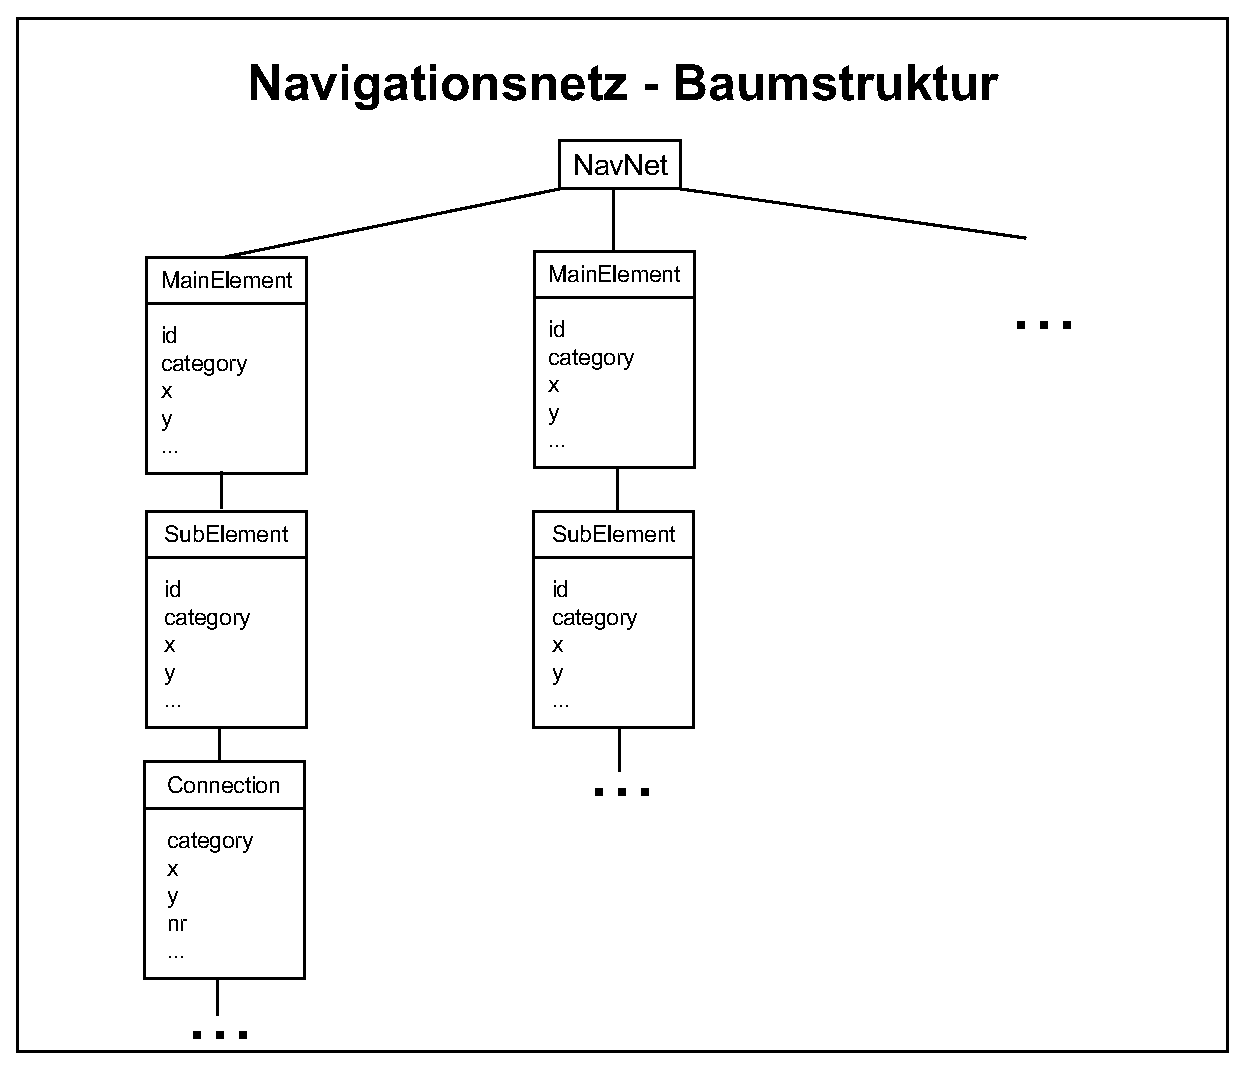
\includegraphics[width=10cm]{figs/baumstruktur}
\captionbelow{Baumstruktur}
\label{FIG:baumstruktur}
\end{figure}
\subsection{Die Layout Klassen} Die Layout
Klassen sind notwendig, um ein Netz �berhaupt darstellen zu k�nnen. In einer
Layout Klasse wird das Aussehen eines Elementes beschrieben, das durch den
Einsatzt von Parametern sehr vielseitig gestaltet werden kann. In einem Skin
werden alle zu einem Thema geh�renden Element in einem Paket zusammengefasst. So
geh�ren die Elemenete MainElement und Connector zum Mathe Skin und geben den
Elementen das Aussehen, wie es in der Mumie Vorgabe spezifiziert ist. So ist es
durch den Einsatz verschiedener Skins m�glich, das Aussehen des Netztes den
jeweiligen Kontexten anzupassen. Es k�nnen nat�rlich auch schon bereits
bestehende Skins benutzt oder erweitert werden. Auf diese Art und Weise wird die
graphische Darstellung von der logischen Struktur des Netzes getrennt. Dadurch
l�sst sich das Applet viel flexibler benutzen und der zu leistende Eigenanteil
beim Entwurf eines neuen Netztes sinkt.
\subsection{Die Zeichen Engine} Im
unmittelbaren Zusammenhang mit den Layout Klassen steht die Zeichen Engine.
Diese ist daf�r verantworlich, das Elemente zum richtigen Zeitpunkt, in der
gew�nschten Reihenfolge an der korrekten Position gezeichnet werden. Ihr ist es
zu verdanken, das jedes Netzt optimal an die Gr�sse des Applets angepasst wird
und Zoom und Tooltips realisiert werden k�nnen. Hinter ihrer Fassade stecken
Berechnungen zur Skalierung und Verschiebung von Punkten, die es erm�glichen,
das Netz auf einem von der realen Ausgabegr�sse unabh�ngigem Raster zu
definieren. Daher muss man sich beim Entwurf eines Neztes keine Gedanken �ber
die Gr�sse der Darstellungsfl�che im Applet und dessen Seitenverh�ltnis zu
machen.
\subsection{Die Event Engine} Die Event Engine ist f�r die Bearbeitung
von Ereignissen und Aktionen zust�ndig. Sie �berpr�ft, ob ein Element angeklickt
wurde und f�hrt im entsprechenden Fall die notwendigen Operationen durch.
Ebenfalls erkennt sie das Benutzen der Zoom Funktion, ermittelt und setzt
notwendige Paramter und veranlasst die Zeichenengine, das Netz gezoomt
darzustellen. Des weiteren veranlasst sie die Einblendung von Tooltips, wenn die
Maus �ber einem Elemnt ruht. Nat�rlich geh�rt die Behandlung der Navigations
Buttons zu ihrem Aufgabengebiet.
\begin{figure}[htbp]
\centering% %\setcapwidth[c]{12cm}%
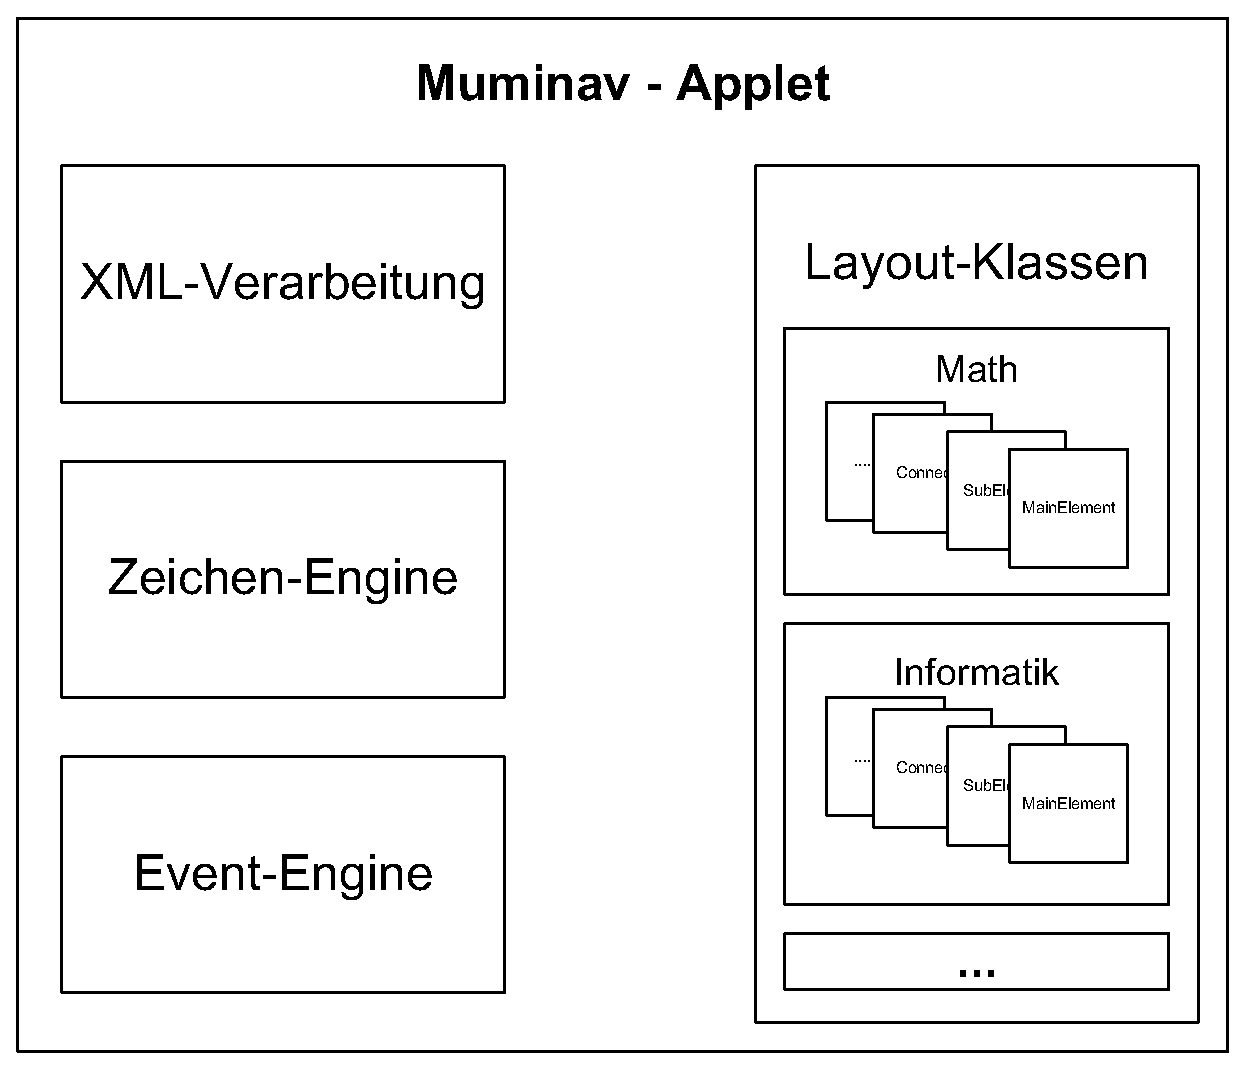
\includegraphics[width=10cm]{figs/aufbau}
\captionbelow{Aufbau: Haupteile von Muminav}
\label{FIG:aufbau}
\end{figure}

\section{Erfahrungen und Probleme}

\subsection{Konzeption und Implementierung}
W�hrend der Arbeit sind f�r ein Projekt solchen Umfangs erstaunlich wenig
Probleme aufgetreten. In den ersten Projektphasen, zeitlich zwischen dem 1. und
3. Meilenstein einzuordnen, haben wir uns fast ausschlisslich mit dem Konzept
besch�ftigt. Diese gr�ndliche Vorbereitung war die Voraussetzung f�r eine recht
komplikationsfreie Implementierungsphase.

Ein gr�sseres Problem stellte die Umsetzung der Tooltips dar. Hier musste ein
angedachter Ansatz verworfen und ein neuer Weg eingeschlagen werden. Eine
Verz�gerung von ca. 2 Tagen war die Folge. Hier kamen die Vorteile der Nutzung
eines CVS Archivs zum Tragen, denn die Verbesserung des Tooltipsystems
beeinflusste nicht die anderen Entwiklung der restlichen Systemteile.

\subsection{Dezentrale Entwicklung}
Sehr angenehm wurde von allen Gruppenmitgliedern der Aspekt und die
Hilfsmittel der dezentralen Entwicklung aufgenommen. Die Konzeptionsphase
gestaltete sich zwar wie gewohnt �ber pers�nliche Treffen, doch lief die gesamte
Entwicklung eigentlich komplett ohne die sonst �blichen Kommunikationsmittel wie
Telefon oder Meetings ab.

Vielmehr setzte sich w�hrend der Implementierungsphase die intensive Nutzung der
Projekt- Mailingliste in Verbindung mit der Nutzung von Instant Messaging durch.
Wir waren alle sehr positiv davon �berrascht, wie gut das funktionierte.

Anfangs hatten wir etwas mit den Eigenheiten von CVS zu k�mpfen. Die Aufteilung
in Module ist uns nicht so gut gelungen, wie es h�tte sein k�nnen. So haben wir
jetzt ein Archiv, in dem redundante Daten liegen, die teilweise nicht mehr
genutzt werden. Hier kann man aber nur f�r die Zukunft lernen und sich vor der
Implementierungsphase noch intensiver mit der Einrichtung der
Entwicklungsumgebung besch�ftigen.

Alles in allem war die Nutzung von CVS eine riesige Zeitersparnis, denn es wurde
uns doch viel Arbeit mit der Koordination der Enwticklung von Programmteilen
abgenommen.

Auch das gemeinsame Schreiben des Abschlussberichtes war uns so m�glich.
\chapter{Beurteilung des Projekts}

\section{Diskussion des Status quo}

\section{Einsatzf�higkeit}

\textsc{Muminav} wurde als hoch spezialisierte Softwarekomponente
f�r den Einsatz im Gesamtprojekt \textsc{Mumie} ins Leben gerufen.
Nichts desto trotz haben wir gro�en Wert darauf gelegt, die
Software so allgemein wie m�glich zu gestalten damit sie f�r
m�glichst viele andere Open-Source-Projekte interessant wird.
Letztendlich wurde, durch den Einsatz von Skins und XML als
Datenformat, aus der Aufgabe, ein Java-Applet zu programmieren,
welches Navigationsnetze f�r Mathematische Kurse im Internet
dynamisch erzeugt, ein Softwaremodul, welches f�r die Darstellung
jeglicher graphischer Darstellungen geeignet ist. Zum Beispiel
lie�en sich leicht Skins erstellen, mit denen man Flowcharts, E/R
Diagramme oder sogar UML darstellen kann.\\
Zus�tzlich ist die Software so ausgelegt, dass sie nicht auf
Applets beschr�nkt ist. Durch das Packaging in ein
Java-Swing-Panel l�sst es sich genau so gut in eine
Java-application einbauen.



\section{Ausblick}

F�r die Zukunft des Projekts haben wir uns vorgestellt, den
Abstraktionsgrad weiter zu steigern, damit es immer leichter wird,
seine eigenen Skins zu entwerfen.\\
Angedacht ist auch ein einfacher Skin-Editor, mit dem man sich
bequem per Maus seine eigenen Skins entwerfen kann.

Interessant w�re es auch, unsere Quelle, die wir bisher auf der
Java-Platform von \textsc{SUN} entwickelt und getestet haben, auf
die Kompatibilit�t zu Open-Source-Kompilern zu testen und
gegebenenfalls anzupassen. Damit k�nnten wir dann auch den
Bytecode unter einer entsprechenden Lizenz ver�ffentlichen.

Wir werden auch versuchen eine kleine Community ins Leben zu
rufen, welche gegenseitig Skins austauscht. Dabei k�nnte man die
\textsc{Muminav}-Homepage zu einem �ffentlich zug�nglichen
Skin-Archiv erweitern, in das jeder seine Skin einbringen und bei
Bedarf von der Kreativit�t anderer profitieren kann.

Was eigentlich gar nicht erw�hnt werden m�sste: \textsc{Muminav},
wie auch jedes andere Open-Source-Projekt, ist mit der
Fertigstellung der ersten Version nicht abgeschlossen. Vielmehr
wird es, solange es aus der Open-Source-Community Interesse und
Anregungen gibt, sich weiterentwickeln. Sei es durch entdeckte
Bugs oder Vorschl�ge f�r neue Features, die durch uns oder
Mitglieder aus der Open-Source-Community in das Projekt
einflie�en.

%--------------------------------------------------------------------


\bibliographystyle{bibstyle} % mit custom-bib erzeugter individueller Bibliographie-Style !!
\bibliography{bibliographie}


\end{document}
